\section{Basisdata}
Basisdata adalah kumpulan data yang terorganisir dan terstruktur yang dirancang untuk menyimpan, mengelola, dan mengubah data secara efektif. Database memungkinkan berbagai tugas seperti pencarian, pembaruan, dan penghapusan data, serta menyediakan penyimpanan data dalam format yang mudah diakses dan dikelola. Database biasanya terdiri dari tabel yang terdiri dari baris dan kolom, dan setiap tabel berisi informasi tentang entitas tertentu. Sebuah tabel yang menyimpan informasi tentang pelanggan, misalnya, mungkin berisi nama, alamat, dan nomor telepon pelanggan. Pengguna dapat melakukan operasi SQL untuk berinteraksi dengan data yang tersimpan dalam database dengan menggunakan sistem manajemen basisdata \citep{santoso2021sql}.

\section{\textit{Entity Relationship Diagram}}
Entity Relationship Diagram (ERD) adalah komponen penting dalam bidang desain database, yang berfungsi sebagai representasi visual dari struktur data dan hubungan antara berbagai entitas dalam suatu sistem. Menurut \citet{bagui2023database}, diagram ER berperan penting dalam pemodelan data, memberikan kerangka kerja yang jelas untuk memahami bagaimana elemen data berinteraksi dan berhubungan satu sama lain dalam lingkungan database.

\begin{figure}[htbp]
  \centering
  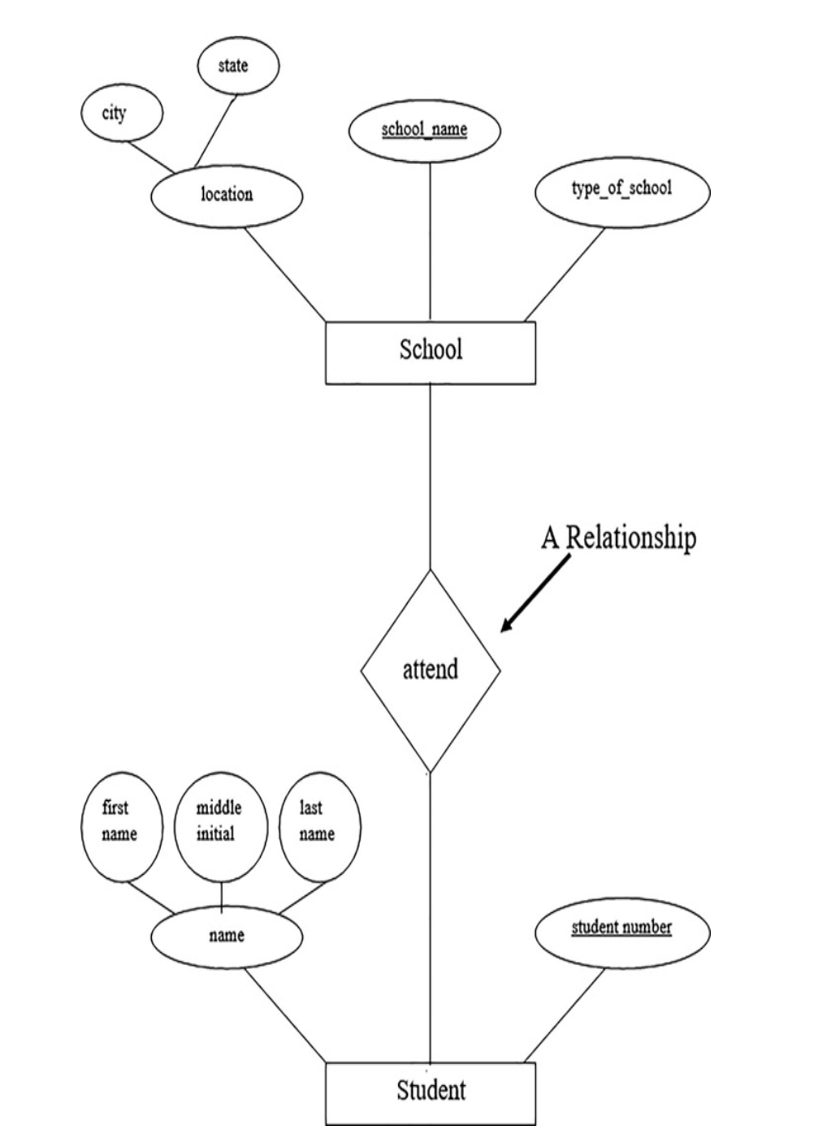
\includegraphics[width=0.85\linewidth]{images/bab-2/erd-example.png}
  \caption{Contoh \emph{ERD}}\label{fig:erd-example}\citep{bagui2023database}
\end{figure}

Elemen utama diagram ER mencakup entitas, atribut, dan hubungan. Entitas didefinisikan sebagai objek atau konsep yang memiliki keberadaan berbeda dan dapat diidentifikasi dalam domain yang diminati. Misalnya, dalam database universitas, entitas mungkin menyertakan ``Mahasiswa'', ``Kursus'', dan ``Instruktur''. Setiap entitas dicirikan oleh atributnya, yang merupakan properti spesifik atau rincian yang menggambarkan entitas tersebut. Misalnya, entitas ``Pelajar'' mungkin memiliki atribut seperti ``ID Pelajar'', ``Nama'', dan ``Tanggal Lahir'' \citep{bagui2023database}.

Relasi dalam diagram ER menggambarkan bagaimana entitas saling berhubungan. Mereka dapat diklasifikasikan berdasarkan jumlah entitas yang terlibat: hubungan unary (satu entitas), biner (dua entitas), dan ternary (tiga entitas). Contoh umum dari hubungan biner adalah antara \"Siswa\" dan \"Kursus\", yang menunjukkan bahwa seorang siswa dapat mendaftar di beberapa kursus, sementara setiap kursus dapat memiliki beberapa siswa yang terdaftar \citep{bagui2023database}. Hubungan dua arah ini penting untuk memodelkan interaksi dalam database secara akurat.

Model ER sangat dihargai karena sifatnya yang intuitif, sehingga dapat diakses oleh pemangku kepentingan teknis dan non-teknis. Ini memberikan cara mudah untuk memvisualisasikan kebutuhan dan hubungan data, yang sangat penting untuk desain database yang efektif \citep{bagui2023database}. Namun, terlepas dari kelebihannya, beberapa pendidik mencatat bahwa siswa sering kesulitan dalam menerapkan konsep ER pada skenario dunia nyata, sehingga menyoroti perlunya contoh dan latihan praktis dalam pengajaran \citep{bagui2023database}.

Kesimpulannya, diagram ER adalah alat dasar dalam desain database, memfasilitasi pemahaman struktur dan hubungan data. Mereka berfungsi sebagai jembatan antara desain konseptual database dan implementasi fisiknya, memastikan bahwa database akhir memenuhi kebutuhan informasi penggunanya.

\section{\textit{SQL}}
Structured Query Language adalah bahasa yang digunakan untuk mengelola dan memanipulasi data dalam sistem manajemen basis data relasional. SQL memungkinkan pengguna untuk melakukan berbagai operasi, seperti pengambilan data, pembaruan, decreasing, dan penghapusan data, serta mendefinisikan struktur data dan mengelola akses ke data tersebut. SQL merupakan standar industri yang diadopsi secara luas untuk interaksi dengan basis data \citep{santoso2021sql}.
\citet{santoso2021sql} menjelaskan berbagai jenis perintah SQL yang dikelompokkan ke dalam beberapa kategori utama, yaitu DDL, DML, DCL, dan lainnya. Berikut adalah penjelasan singkat mengenai masing-masing kategori:
\begin{enumerate}
  \item DDL (Data Definition Language): DDL digunakan untuk mendefinisikan struktur database. Perintah-perintah dalam DDL termasuk:
        \begin{itemize}
          \item ``CREATE'': untuk membuat objek database seperti tabel, indeks, dan skema.
          \item ``ALTER'': untuk mengubah struktur objek yang sudah ada.
          \item ``DROP'': untuk menghapus objek dari database.
        \end{itemize}
        DDL berfokus pada bagaimana data disimpan dan diorganisir dalam database.
  \item DML (Data Manipulation Language): DML digunakan untuk mengelola data dalam objek database. Perintah-perintah dalam DML termasuk:
        \begin{itemize}
          \item ``SELECT'': untuk mengambil data dari tabel.
          \item ``INSERT'': untuk menambahkan data baru ke dalam tabel.
          \item ``UPDATE'': untuk memperbarui data yang sudah ada.
        \end{itemize}
        DML berfokus pada manipulasi data yang ada dalam database.
  \item DCL (Data Control Language): DCL digunakan untuk mengontrol akses ke data dalam database. Perintah-perintah dalam DCL termasuk:
        \begin{itemize}
          \item ``GRANT'': untuk memberikan hak akses kepada pengguna atau peran tertentu.
          \item ``REVOKE'': untuk mencabut hak akses yang telah diberikan.
        \end{itemize}
        DCL berfokus pada keamanan dan kontrol akses terhadap data.
  \item TCL (Transaction Control Language): TCL digunakan untuk mengelola transaksi dalam database. Perintah-perintah dalam TCL termasuk:
        \begin{itemize}
          \item ``COMMIT'': untuk menyimpan semua perubahan yang dilakukan dalam transaksi.
          \item ``ROLLBACK'': untuk membatalkan perubahan yang belum disimpan.
          \item ``SAVEPOINT'': untuk menetapkan titik pemulihan dalam transaksi.
        \end{itemize}
        TCL berfokus pada pengelolaan transaksi untuk memastikan integritas data.
\end{enumerate}

\section{\textit{PostgreSQL}}
PostgreSQL adalah sistem basis data objek-relasional sumber terbuka yang kuat, yang memperluas bahasa SQL dengan berbagai fitur untuk menangani beban kerja data yang kompleks dengan aman dan efisien. Pengembangan PostgreSQL dimulai pada tahun 1986 sebagai bagian dari proyek POSTGRES di Universitas California, Berkeley, dan telah mendapatkan lebih dari 35 tahun pengembangan aktif pada platform intinya.
\singlespacing{}
Dikenal karena arsitekturnya yang andal, integritas data, fitur-fitur yang luas, dan fleksibilitas, PostgreSQL didukung oleh komunitas sumber terbuka yang berdedikasi untuk memberikan solusi inovatif dan berkinerja tinggi secara konsisten. PostgreSQL kompatibel dengan semua sistem operasi utama, telah mematuhi standar ACID sejak tahun 2001, dan menawarkan ekstensi yang kuat seperti PostGIS yang populer untuk data geospasial. Oleh karena itu, tidak mengherankan bahwa PostgreSQL telah menjadi basis data relasional sumber terbuka pilihan bagi banyak individu dan organisasi \citep{postgresql2025}.

\section{\textit{NoSQL}}
NoSQL (sering diartikan sebagai ``Not Only SQL'') mengacu pada kelas teknologi penyimpanan data non-relasional yang dirancang untuk mengatasi keterbatasan pada basis data relasional tradisional, terutama dalam konteks aplikasi modern, bervolume tinggi, dan berubah dengan cepat. Tidak seperti sistem berbasis SQL, basis data NoSQL tidak memerlukan skema yang kaku dan dapat secara efisien menangani data semi-terstruktur atau tidak terstruktur \citep[hal.~3]{suehring2021redis}.
\singlespacing{}
Ada empat jenis utama basis data NoSQL{:} penyimpanan \emph{key-value}, penyimpanan dokumen, penyimpanan \emph{wide-column}, dan basis data grafik. Masing-masing dioptimalkan untuk kasus penggunaan yang berbeda-misalnya, penyimpanan \emph{key-value} ideal untuk pencarian cepat, sedangkan basis data grafik cocok untuk aplikasi dengan hubungan yang kompleks seperti jejaring sosial \citep[hal.~4-5]{suehring2021redis}.
Basis data NoSQL sangat berguna ketika aplikasi membutuhkan:
\begin{itemize}
  \item Performa tinggi di bawah beban data berskala besar,
  \item Fleksibilitas skema,
  \item Skalabilitas horizontal melalui sharding,
  \item Ketersediaan tinggi dan toleransi kesalahan \citep[hal.~6-7]{suehring2021redis}.
\end{itemize}


Tidak seperti basis data relasional yang biasanya membutuhkan gabungan yang rumit dan skema yang dinormalisasi, NoSQL menawarkan model yang lebih ramah pengembang. Hal ini penting untuk praktik pengembangan yang gesit di mana model data dapat berkembang dari waktu ke waktu \citep[hal.~6]{suehring2021redis}.

\subsection{Redis}
Redis adalah database NoSQL in-memory sumber terbuka yang menawarkan performa luar biasa cepat dengan menyimpan data terutama di RAM, dengan disk persistence opsional untuk durabilitas \citep[p.~7]{suehring2021redis}. Meskipun Redis sering dikategorikan sebagai key-value store, sebenarnya Redis adalah database multi-model, yang mampu menyimpan dan memanipulasi berbagai struktur data seperti:
\begin{itemize}
  \item Strings
  \item Lists
  \item Sets
  \item Hashes
  \item Sorted Sets
  \item Streams
  \item Geospatial data
  \item Bitmaps dan HyperLogLogs \citep[pp.~32-38]{suehring2021redis}
\end{itemize}
\singlespacing{}
Redis mendukung messaging Pub/Sub, analitik real-time, manajemen sesi, dan pelacakan leaderboard, menjadikannya ideal untuk aplikasi web dan seluler modern yang menuntut interaktivitas real-time \citep[pp.~11-15]{suehring2021redis}.
\singlespacing{}
Selain itu, Modul Redis memperluas kemampuannya untuk mencakup fitur-fitur seperti pencarian teks lengkap (melalui RediSearch), analisis time-series (RedisTimeSeries), dan querying graph (RedisGraph), memungkinkan Redis untuk mendukung pola akses data multi-model tanpa lapisan kompleksitas tambahan \citep[pp.~41-43]{suehring2021redis}. Karena sifat in-memory dan struktur data yang dioptimalkan, Redis menawarkan waktu respons sub-millisecond dan throughput yang luar biasa, sehingga cocok tidak hanya untuk caching tetapi juga sebagai database utama dalam skenario kinerja tinggi \citep[p.~12]{suehring2021redis}.
\singlespacing{}
Redis juga unggul dalam high availability dan kasus penggunaan sistem terdistribusi, mendukung replikasi, clustering, dan mekanisme automatic failover, sehingga menjadikannya siap produksi untuk aplikasi-aplikasi kritis \citep[p.~46]{suehring2021redis}.